\documentclass[12pt, a4paper]{article}
\setlength{\parindent}{0pt}
\usepackage[a4paper, portrait, margin=1in]{geometry}
\usepackage{graphicx}

\graphicspath{.}

\usepackage{preamble}

\begin{document}

\textbf{(Q3)}

\begin{proof}

\textit{(a)(i)}

We can sketch such a partition as shown:

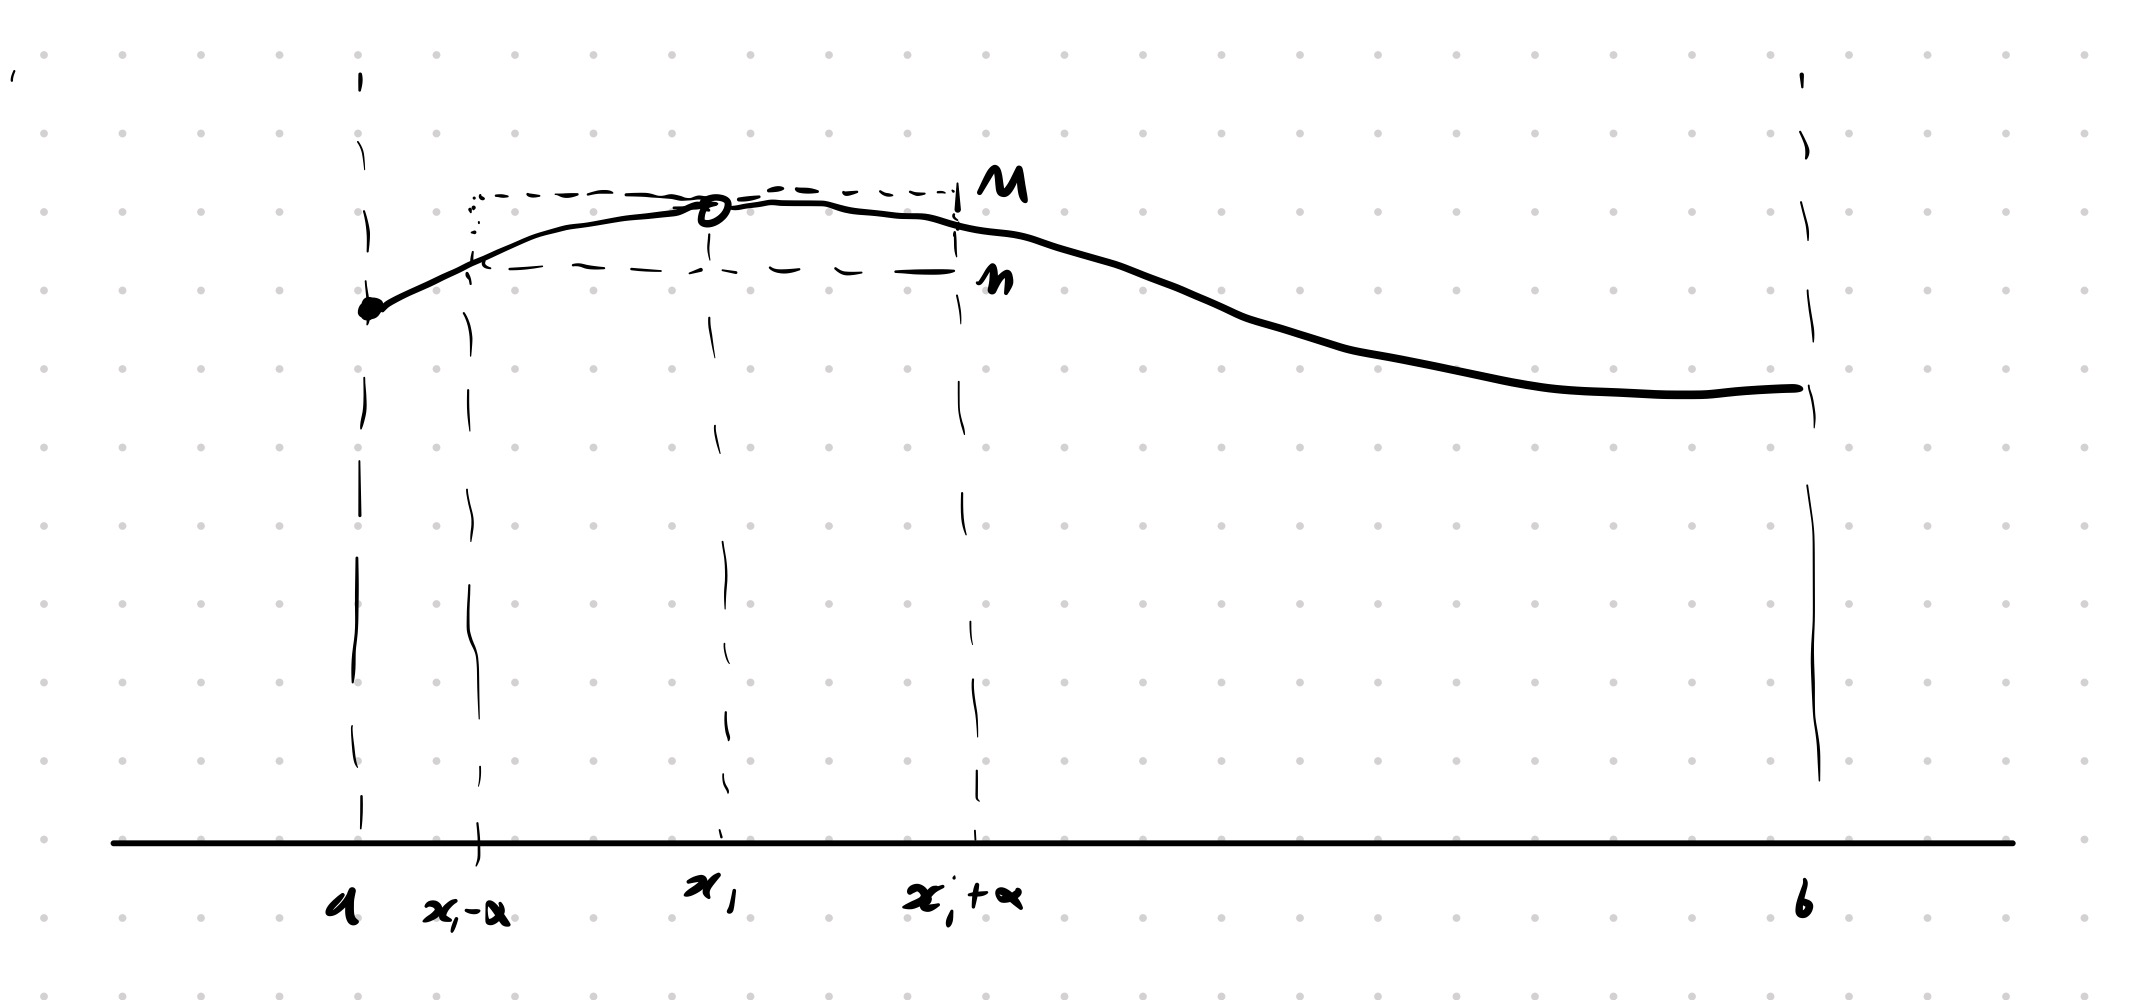
\includegraphics[width=\textwidth]{q3sketch.jpg}

\textit{(a)(ii)} We observe that $\Delta x = 2\alpha$. Then we want to show:

\[
    M \Delta x - m \Delta x = 2 \alpha (M - m) \leq \frac{\varepsilon}{3}
\]

Since $M$ and $m$ are dependent on $\alpha$, set $\alpha$ such that
$\alpha = \min \{M - m \leq \frac{1}{3}, \frac{\varepsilon}{2}\}$.

Then we have

\[
    2 \alpha (M - m) \leq \frac{1}{3} \cdot \varepsilon
    = \frac{\varepsilon}{3}
\]

\textit{(a)(iii)} Since $f$ is continuous on $[a, x_1 - \alpha]$ and
$[x_1 + \alpha, b]$, it is integrable and thus fulfils the
$\varepsilon$-characterization of integrability:

\begin{gather*}
    \exists P_1 \st U_{P_{1}} - L_{P_{1}} < \frac{\varepsilon}{3}\\
    \exists P_2 \st U_{P_{2}} - L_{P_{2}} < \frac{\varepsilon}{3}
\end{gather*}

\textit{(a)(iv)} Hence, we have:

\[
    2 \alpha (M - m) + U_{P_{1}} - L_{P_{1}} + U_{P_{2}} - L_{P_{2}} < \varepsilon
\]

Which fulfils the $\varepsilon$-characterization of integrability and thus
satisfies the base case.

\textit{(b)(i)} Again, since $f$ is continuous on $[a, x_N - \alpha]$
and $[x_N + \alpha, b]$, it fulfills the $\varepsilon$-characterization
of integrability.

\textit{(b)(ii)} We refer to $(a)(ii)$ to confirm that this holds.

\textit{(b)(iii)} Thus, for arbitrary $N$, we have:

\[
    2 \alpha (M - m) + U_{P_{1}} - L_{P_{1}} + U_{P_{2}} - L_{P_{2}} < \varepsilon
\]

And so the induction hypothesis holds.

\end{proof}

\end{document}